\documentclass{article}

\usepackage{arxiv}

\usepackage[utf8]{inputenc} % allow utf-8 input
\usepackage[T1]{fontenc}    % use 8-bit T1 fonts
\usepackage{hyperref}       % hyperlinks
\usepackage{url}            % simple URL typesetting
\usepackage{booktabs}       % professional-quality tables
\usepackage{amsfonts}       % blackboard math symbols
\usepackage{nicefrac}       % compact symbols for 1/2, etc.
\usepackage{microtype}      % microtypography
%\usepackage{cite}
\usepackage{natbib}
\usepackage{graphicx}
\usepackage{booktabs}

\title{Belief Polarization: An Agent-Based Modeling Approach (Proposal)}


\author{
  Brian Lubars \\
  \texttt{brian.lubars@colorado.edu} \\
   \And
  Peter Innes \\
  \texttt{peter.innes@colorado.edu} \\
  \And
  Sierra Jech \\
  \texttt{sierra.jech@colorado.edu}
}

\begin{document}
\maketitle

%\begin{abstract}
%\lipsum[1]
%\end{abstract}

\section{Introduction}
The phenomenon of ideological polarization has become a topic of increasing national and international concern in the past several decades. Marked by waves of nationalist political movements that clash with progressive, liberal politics, polarization can render governments ineffective (i.e. the recent U.S. government shutdown), as animosity grows between political factions and chances of compromise diminish \citep{party_loathing}. While it may be easy to blame bureaucrats for yelling across the aisle to no avail, the problem of polarization is rooted throughout American society. Opinions regarding divisive issues such as abortion, health care, and immigration, have increasingly become tied to personal identity and ultimately factor into where we choose to live and who we choose to surround ourselves with, both in-person and online \citep{polarized_society}.

Along these lines, social media allows rapid and unmediated dissemination of information (i.e. Facebook) and provides an arena for identity politics to play out in the public sphere. Of particular concern is the ability of social media to accelerate the growth of polarized camps of belief that are individually homogeneous, especially via the spread of misinformation \citep{PNASmisinfo}. Essentially, individuals' social networks tend to resemble echo chambers, in which only one type of opinion is amplified \citep{facebook_echo}.

This phenomenon has recently been illustrated by the 2016 U.S. presidential election. Following a heated national debate surrounding the two candidates, Donald Trump and Hillary Clinton, a national investigation has revealed an extensive, Russian-directed social media influence campaign that sought to sew discord, increase polarization, and ultimately undermine the democracy of the United States, in attempt to support Trump's candidacy \citep{russian}.

More than any other recent social or political debate, the Russian interference campaign has  brought to light the power of online social networks in swaying public opinion, especially in regards to ideological polarization. Thus, it is important to develop models of how polarization occurs in online social networks, especially given outside actors, such as media sources--fake or real--so that social media companies can work to prevent insidious use of their platforms.

\subsection{Related Work}

\citet{bramson2017} identify several computational models people have used to reproduce and explain patterns of polarization. We find only a few broad classes of models -- apparently, attempts to naively model imitation and influence of opinion dynamics often lead to belief convergence. Nevertheless, we identify several models from which we have drawn our inspiration: (1) Cultural Diffusion models in which people interact more with those similar to themselves while becoming more similar to those they interact with; (2) Bounded Confidence models, wherein agents update their opinions to be an average of those within a certain threshold of themselves; and (3) Structural Balance Theory-based models, wherein certain social triad configurations are stable and others are unstable \citep{bramson2017}. 

Group polarization, in social psychology, is the tendency for a group of individuals to reach more extreme positions than the group's members might individually. Confirmation bias is one possible mechanism, and this has been successfully modeled using a continuous variation of the Bounded Confidence Model called the Unbounded Confidence Model (UCM), along with negative feedback wherein an agent's belief may update towards the opposite of its neighbor \citep{confbias}. \citet{confbias} also consider rewiring the social network, but find two stable polarized groups are possible with just the UCM.

Scientists can sometimes become polarized into camps of competing theories, as in the scale-free networks and preferential attachment debates in complex networks \citep{scalefree}. \citet{oconnor2017} present a model of scientific polarization in which agents become polarized even when agents rationally gather evidence about their beliefs to maximize their probability of finding the ``truth''. The mechanism responsible is treating evidence as more uncertain when it comes from agents with beliefs different from your own \citep{oconnor2017}.

A related family of models, which we decided not to purse, consider information spreading through a network according to epidemic/percolation models. \citet{misinformation_spread} found polarization and homogeneity are the main factors predicting the size of a cascade of shares on a social network. \citet{hoax_spread} consider the potential impact of fact-checking on information spreading, finding a fact-checking probability that guarantees the eradication of a hoax.  

Last but not least, we must consider the definition of polarization itself. \citet{bramson2017} identify nine metrics for polarization used in various combinations by the above models, and note that there is wide inconsistency in use. In every case, at least one of the metrics decreases under apparent increasing polarization. 
When considering a single dimensional belief along a continuous spectrum, one commonly-used definition is that a more polarized population will show a more bi-modal distribution, with more spread. Other possible metrics are population dispersion, or amount of belief spectrum coverage. 
Group-based metrics also have an intuitive appeal, but it may be problematic to identify groups when their distributions overlap. Examples of group-based metrics include homogeneity of the groups, distinctness, or divergence. Given a network structure and ``ground-truth'' group labels, connectivity between the groups can also measured \citep{bramson2017}. 

\subsection{Research Question and Hypotheses}
\textbf{How do media sources impact polarization of opinions in socially connected individuals?} \hfill\break
\\
\textbf{Hypothesis 1.}  Polarization does not occur when all agents have the same evidence for forming opinions.\\
\textbf{Hypothesis 2.} Polarization occurs when agents have different sources of evidence (media sources) available and cannot update their opinions based on their neighbors. \\
\textbf{Hypothesis 3.} Polarization occurs when agents have access to different sources of evidence and are able to update their opinions based on their neighbors' opinions.\\ 
\textbf{Hypothesis 4.} Amplification of a media source (meddling) will speed polarization of opinions.

\section{Plan of Execution}

To address the above research question and hypotheses, we intend to explore some of the mechanisms behind belief polarization using agent-based modeling. Agents will be connected to each-other through a network, each agent will contain a belief along a spectrum $[-1, 1]$ (initialized uniformly at random), and will iteratively update their belief at every time step, according to a set of local rules (see Figure \ref{fig:fig1}). 

\begin{figure}[ht]
  \centering
  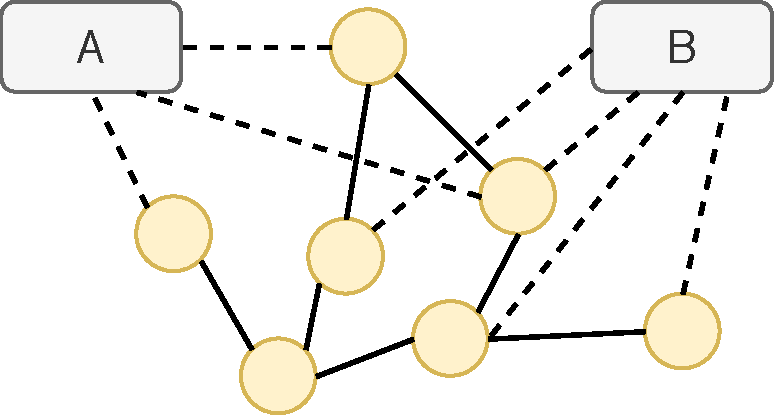
\includegraphics[width=10cm]{pol_network.pdf}
  \caption{Sample network, with 7 agents and 2 media sources (A and B). Agents subscribe to none, one, or several media sources.}
  \label{fig:fig1}
\end{figure}

\subsection{Methods}

We will use NetLogo with the Networks add-on to implement and run the model. Generally, we wish to model how polarization is impacted by different media diets or network structures, how confirmation bias may effect belief formation, and how sensitive any effects are to initial conditions. If we can successfully reproduce polarization under these effects, we also would like to try to understand the effectiveness of possible mitigations, such as specific media diets, less homogeneous connections, or reduced ``propaganda'' visibility. 

\paragraph{Belief Updating}

Specifically, we will try variations of the bounded confidence model imposed over a social network structure (the original model used all agents within a threshold, effectively an all-to-all network). We will simulate the effects of media as special agents with special connections to subsets of the network, such that the media only influences and never updates their beliefs. We will initialize the agents in the network to have random uniformly-distributed beliefs. Then agents will update according to the following local rules:
\begin{enumerate}
    \item For each agent $x_i$: Survey beliefs of all neighbors, including media sources, that are within a threshold $t_i$ of the agent's belief: $B_i = \{belief(x_j) \forall x_j \in neighbor(x_i) s.t. |belief(x_i) - belief(x_j)| \leq t_i \}$
    \item Update agent's belief as the average of that set of beliefs: $belief(x_i) = \frac{1}{|B_i|} \sum_j B_{ij}$
\end{enumerate}

The main drawback of the bounded confidence interval is that boundary effects on the belief spectrum range [-1, 1] mean that agents are typically pulled away from the extremes towards the center. This effect would seem to be dissimilar to the effects from confirmation bias, from which we might expect the same evidence to cause two camps to diverge further in belief. 

To account for this, we would like to explore a second set of local rules for agent belief updating, similar to \citet{confbias}. Under Bounded Confidence rules, people would update their beliefs to be the average of all the beliefs they can see which are within a certain threshold. Instead, we may consider \textbf{evidence} to be shared, and people instead update their beliefs according to their perception of the evidence. This allows for the inclusion of confirmation bias into the belief dynamics, since agents may now consider both the evidence and the position of the people who shared the evidence when updating their beliefs. A possible extension could also consider the beliefs of those people sharing it (evidence coming from a potentially biased source).
\begin{enumerate}
    \item For each agent $x_i$: Survey evidence shared by neighbors
    \item Update belief based on some function $f$ of own belief, others beliefs, and evidence: $belief(x_i) = \frac{1}{n} \sum_j f(belief(x_i), belief(x_j), evidence_j)$
\end{enumerate}

\paragraph{Evaluation.} There are several proposed methods to quantitatively measure the amount of polarization \citep{oconnor2017}. We propose using statistical measures of the \textbf{spread}/variance or average distance between opinion values and \textbf{homogeneity}, a measure of the within-group similarity in opinion values.

\paragraph{Stochastic Block Model.} We are also curious about the effects of network structure on polarization. To explore this we can generate random networks with various degrees of community structure using the stochastic block model. We can then run our local agent update rules and determine how varying the  community strength impacts the population's polarization, and how closely any emergent belief groups might align with the natural community structures.

\paragraph{Propaganda.} Russian media influence during the election was found to take two main forms \citep{russian}:
\begin{itemize}
\item Creation of new stories, using Russian media such as RT or fake news sites
\item Amplification/spread of existing stories using bots on twitter
\end{itemize}
We can simulate the effects on a network by representing propaganda efforts as a new media source with an extreme position, with more or fewer connections into the network of belief-updating agents. 

\subsection{Timeline}
A timeline of activities for this project are shown in Table \ref{tab:timeline}. Implementation includes writing code, testing the model, and making adjustments and improvements. We anticipate the initial model building to take up the majority of the project time. Trying and testing different methods and ideas will make up the bulk of what will be formally discussed in the presentation and paper. 

\begin{table}[ht]
 \caption{Project timeline}
  \centering
\begin{tabular}{@{}ll@{}}
\toprule
\textbf{Week} & \textbf{Description}                                                         \\ \midrule
1             & Implement model framework in NetLogo                                         \\
2             & Test belief updating method 1                                                \\
3             & Test belief updating method 2                                                \\
4             & Try community structure                                                      \\
5             & Assemble results \& build presentation                                       \\
-             & \begin{tabular}[c]{@{}l@{}}(Presentation May 1)\\ (Paper May 9)\end{tabular} \\ \bottomrule
\end{tabular}
  \label{tab:timeline}
\end{table}

\section{Future Work}
This model has the potential to address many questions beyond those proposed above. While we are using a static network to model social connections, it would make sense to modify the network edges dynamically as individuals add or drop friends according to changing opinions.  It would also make sense to include multiple opinions, representing different issues, similar to approaches in cultural diffusion models \citep{bramson2017}. Our proposed model uses a single value to represent the individual's opinion, but this could be made more complex. Future work could incorporate group polarization theory which includes several different ideas about how groups may converge to an opinion that is more polarized than the average of the individuals \citep{yardi_twitter}. In general, all of these options for future work aim to address opinion polarization in social networks where opinions are based on both evidence (media sources) and the beliefs of those in your immediate social network. This is a first step to determining vulnerabilities in the democratic process that may be exploited now and in the future.


\bibliographystyle{plainnat}
\bibliography{references}

\end{document}
